\documentclass[a4paper,10pt,landscape,twocolumn]{scrartcl}

%% Settings
\newcommand\problemset{4}
\newcommand\deadline{Thursday, 14 September 2017, 20:00h}
\newcommand\worksession{Friday, 15 September 2017}
\newif\ifcomments
\commentsfalse % hide comments
%\commentstrue % show comments

%% Packages
\usepackage[english]{exercises}
\usepackage{wasysym}
\usepackage{graphicx}
\usepackage{hyperref}
\hypersetup{colorlinks=true, urlcolor = blue, linkcolor = blue}
\usepackage{enumitem}

%% Macros
\usepackage{xspace}

\newcommand{\eps}{\varepsilon}
\newcommand{\ket}[1]{|#1\rangle}
\newcommand{\bra}[1]{\langle#1|}
\newcommand{\inp}[2]{\langle{#1}|{#2}\rangle}
\newcommand{\norm}[1]{\parallel\!#1\!\parallel}
\newcommand{\points}[1]{\marginpar{\textbb{#1 p.}}}
\newtheorem{theorem}{Theorem}
\newtheorem{definition}{Definition}
\newtheorem{proposition}{Proposition}
%\newenvironment{proof}{\noindent {\bf Proof }}{{\hfill $\Box$}\\}

\newcommand{\gen}{\ensuremath{\mathsf{Gen}}\xspace}
\newcommand{\enc}{\ensuremath{\mathsf{Enc}}\xspace}
\newcommand{\dec}{\ensuremath{\mathsf{Dec}}\xspace}
\newcommand{\mac}{\ensuremath{\mathsf{Mac}}\xspace}
\newcommand{\vrfy}{\ensuremath{\mathsf{Vrfy}}\xspace}
\newcommand{\negl}{\ensuremath{\mathsf{negl}}\xspace}
\newcommand{\PrivK}{\ensuremath{\mathsf{PrivK}}\xspace}
\newcommand{\eav}{\ensuremath{\mathsf{eav}}\xspace}

\newcommand{\Z}{\ensuremath{\mathbb{Z}}}
\newcommand{\R}{\ensuremath{\mathbb{R}}}
\newcommand{\N}{\ensuremath{\mathbb{N}}}


\newcommand\floor[1]{\lfloor#1\rfloor}
\newcommand\ceil[1]{\lceil#1\rceil}

% \newcommand{\comment}[1]{{\sf [#1]}\marginpar[\hfill !!!]{!!!}}
\newcommand{\chris}[1]{\comment{\color{blue}Chris: #1}}
\newcommand{\jan}[1]{\comment{\color{magenta}Jan: #1}}


\begin{document}

\problems

{\sffamily\noindent
We will work on the following exercises together during the work sessions on \worksession.

You are strongly encouraged to work together on the exercises, including the homework. You do not have to hand in solutions to these problem sets.}

\begin{exercise}[not PRGs]
For all of the following constructions, explain why they are not PRGs. If necessary, give an explicit description of an efficient distinguisher.

\begin{subex}
Let $G(s)$ output $s$.
\end{subex}

\begin{subex}
Let $G(s)$ output $s \| s$
\end{subex}

\begin{subex}
Let $G(s)$ output $s \| \bigoplus_{i=1}^n s_i$.
\end{subex}

\end{exercise}

\begin{exercise}[Basic properties of PRGs]
Recall that the \href{https://en.wikipedia.org/wiki/Image_(mathematics)}{\emph{image} of a function} $f:A \rightarrow B$ is the subset $f(A)$ of $B$. Formally, 
\[ \mathsf{im}(f) := f(A) = \{b \in B \mid \exists a \in A \mbox{ such that } b=f(a) \} \, .
\]

Let $G:\{0,1\}^n \rightarrow \{0,1\}^{2n}$ be a PRG. 

\begin{subex}
Let us assume that $G$ is \href{https://en.wikipedia.org/wiki/Injective_function}{injective}. How many different $2n$-bit strings $y$ are there in the image of $G$?
\end{subex}

\begin{subex}
What is the fraction of images of $G$ among all $2n$-bit strings?
\end{subex}

\begin{subex}
For a given $y \in \{0,1\}^{2n}$, what is $\Pr_{s \leftarrow \{0,1\}^n}[G(s) = y]$? Express it in terms of $|\{s \in \{0,1\}^n \mid G(s)=y\} |$ and $n$.
\end{subex}

\end{exercise}

\begin{figure}[h]
\center
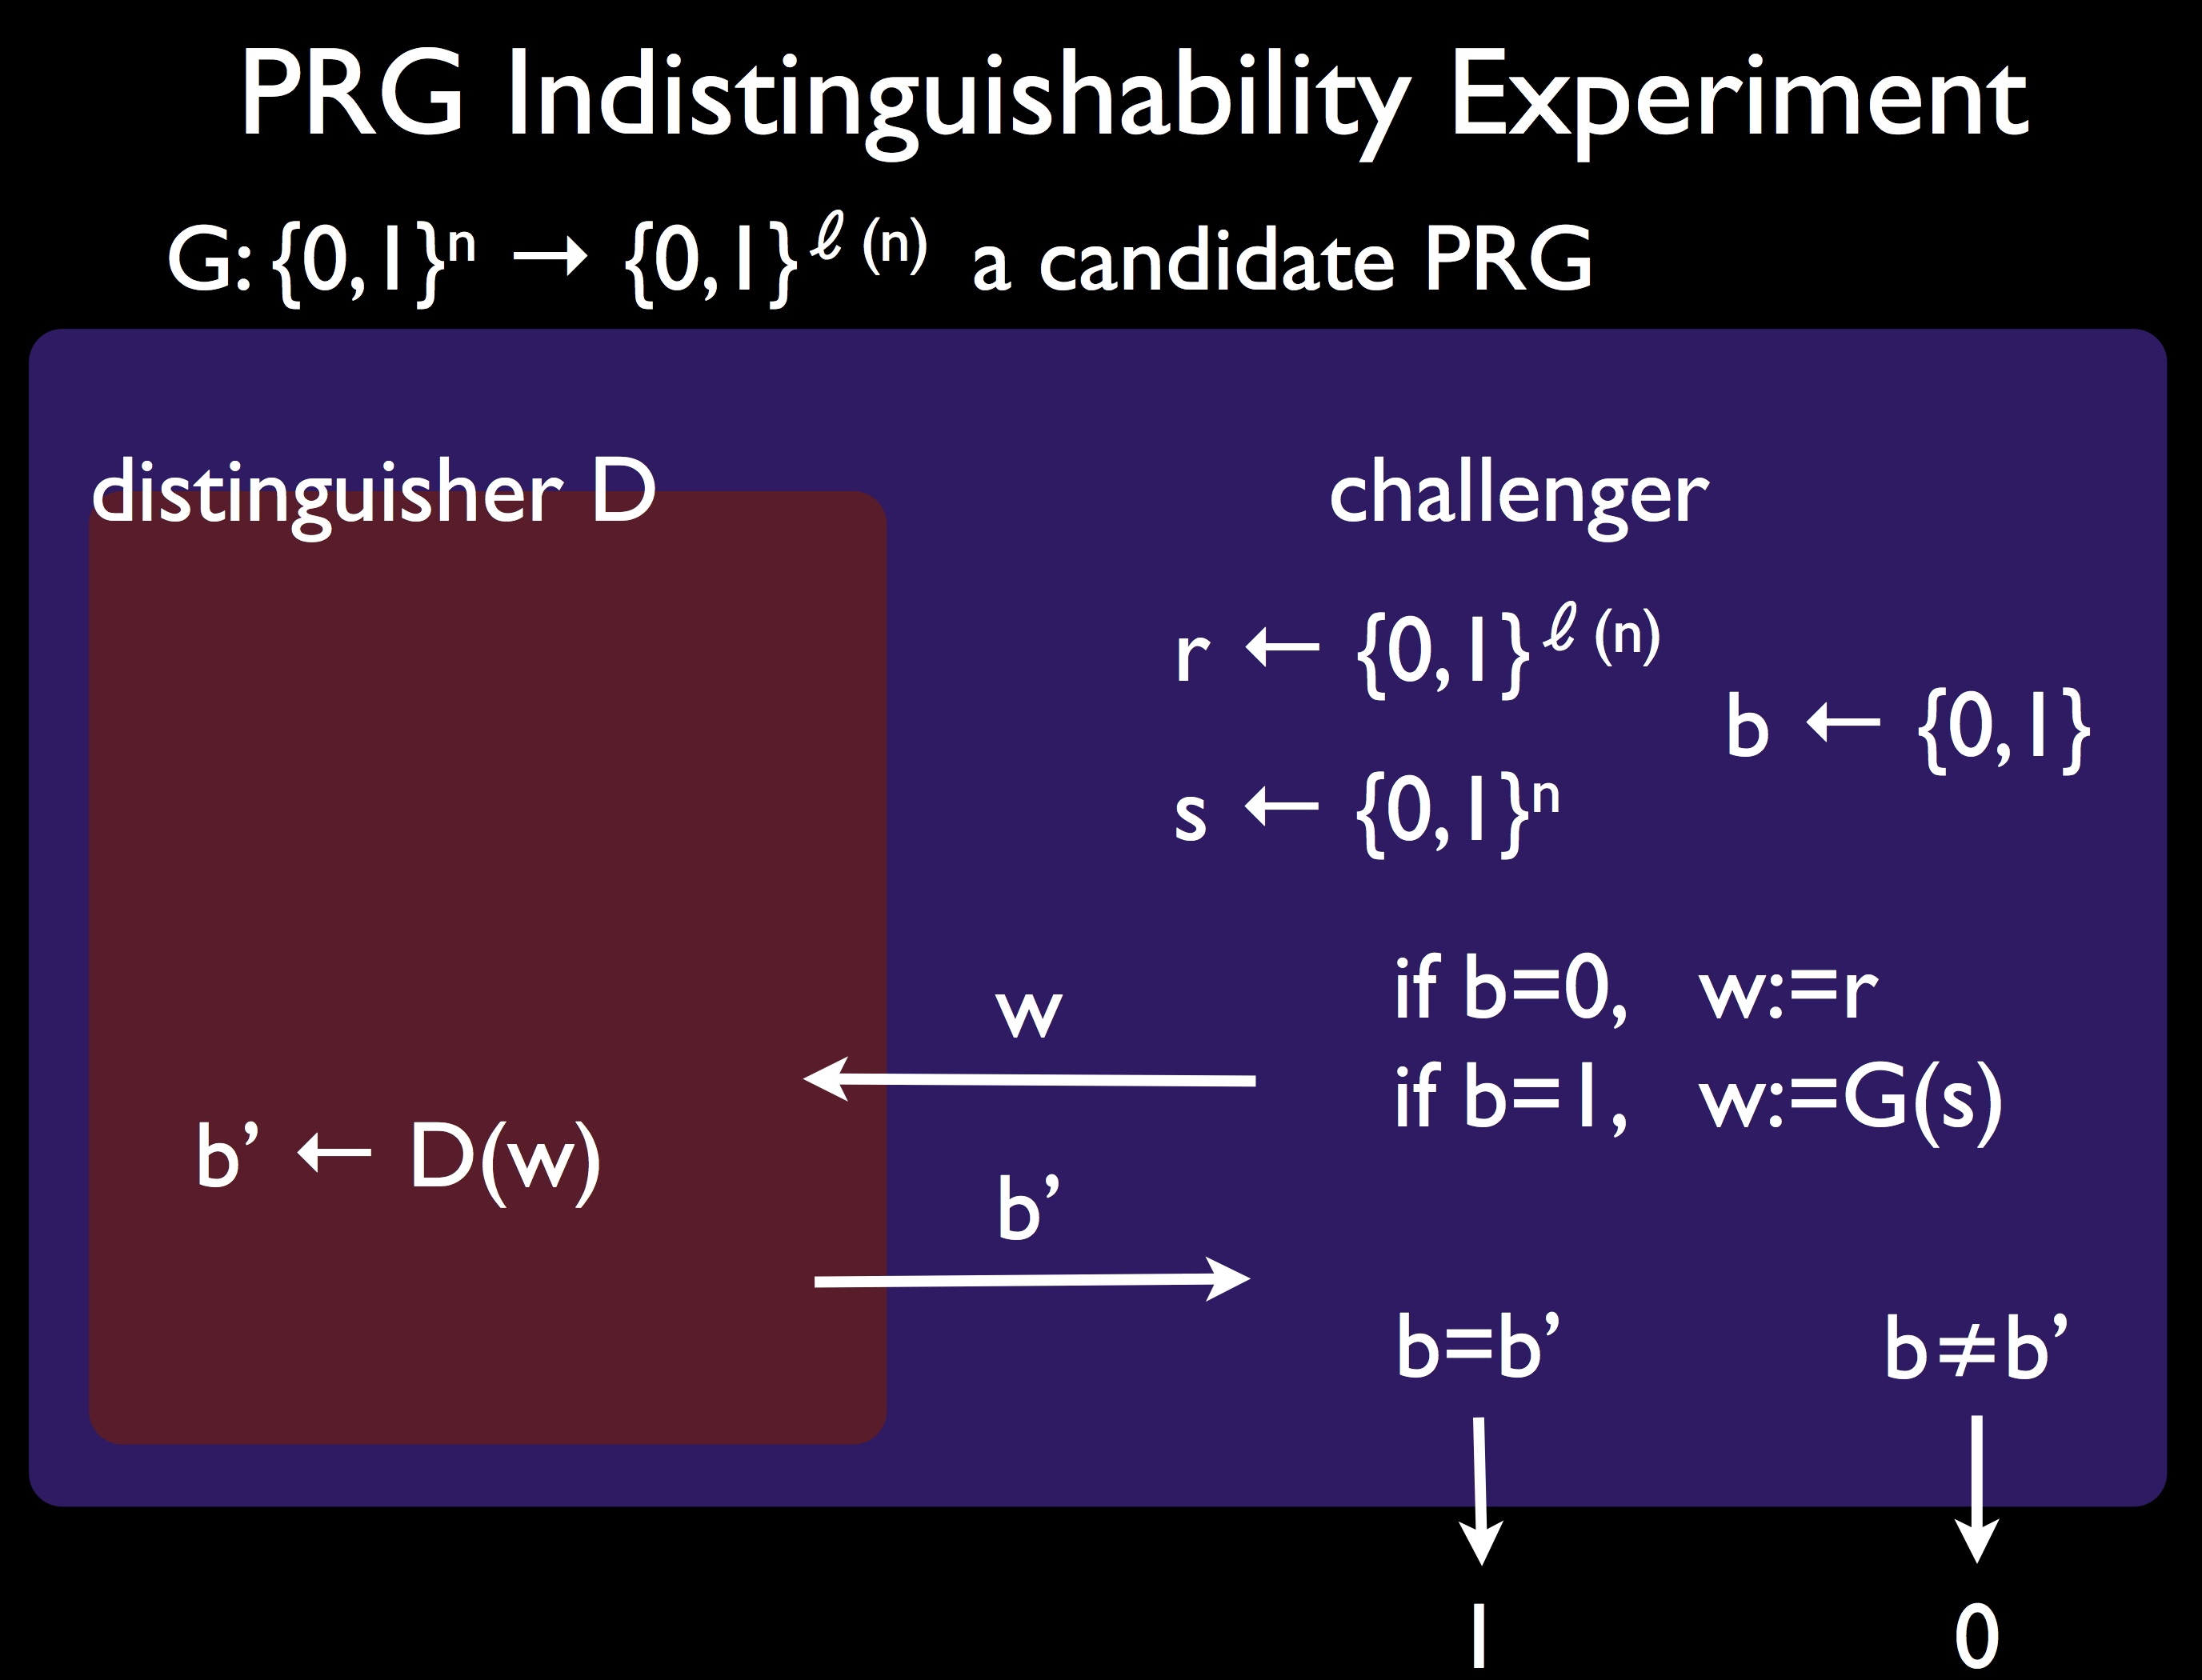
\includegraphics[width=8cm]{PRGExperiment.jpg}
\caption{The $\mathsf{PRG}_{\mathcal{A},G}$ experiment \label{fig}}
\end{figure}

\begin{exercise}[Exercise~3.5 from  $\text{[KL]}$ ]
  Let $|G(s)| = \ell(|s|)$ for some $\ell$. Consider the following experiment:

  \textbf{The PRG indistinguishability experiment} $\mathsf{PRG}_{\mathcal{A},G}(n)$, see also Figure~\ref{fig}:
  \textit{
  \begin{enumerate}[label=(\alph*)]
\item  A uniform bit $b \in \{0,1\}$ is chosen. If $b = 0$ then choose a uniform $r \leftarrow \{0, 1\}^{\ell(n)}$ and set $w:=r$; if $b = 1$ then choose a uniform $s \leftarrow \{0,1\}^n$ and set $w := G(s)$.
\item The adversary $\mathcal{A}$ is given $w$, and outputs a bit $b'$.
\item The output of the experiment is defined to be 1 if $b' = b$,
  and 0 otherwise.
  \end{enumerate}
  }
Provide a definition of a pseudorandom generator based on this experiment, and prove that your definition is equivalent to Definition 3.14. (That is, show that $G$ satisfies your definition if and only if it satisfies Definition 3.14.)
  
\end{exercise}

\pagebreak
\begin{exercise}[Brute-forcing a PRG]
Let $G:\{0,1\}^n \rightarrow \{0,1\}^{2n}$ be a PRG. Describe a \emph{computationally unbounded} adversary $\mathcal{A}$ that distinguishes the output of $G$ from a uniform $2n$-bit string with probability exponentially close 1. How does it work? Compute its exact distinguishing advantage. What is $\Pr[\mathsf{PRG}_{\mathcal{A},G}(n)=1]$ for this adversary?
\end{exercise}

\begin{bonusexercise}[Exercise~3.7 from $\text{[KL]}$ ]
Prove the converse of Theorem 3.18. Namely, show that if $G$ is not a pseudorandom generator then Construction 3.17 does not have indistinguishable encryptions in the presence of an eavesdropper.
\end{bonusexercise}

  


\end{document}
